\documentclass[11pt]{article}
\usepackage[utf8]{inputenc}
\usepackage{amsmath}
\usepackage{amssymb}
\usepackage{tikz}
\usepackage{circuitikz}
\usepackage[toc,page]{appendix}
\usepackage{pdfpages}
\usepackage{epstopdf}
\usepackage{amssymb}
\usepackage{subcaption}
\usepackage{siunitx}
\usepackage{url}
\usepackage{minted}
\usepackage{tabularx}
\usepackage{svg}
\usepackage{wrapfig}
\usepackage{bm}
\usepackage[export]{adjustbox}


\usemintedstyle{solarizedlight}
\input{solarizedlight.pygstyle}

\setminted{
    linenos,
    breaklines,
    fontsize=\small,
}

\usepackage{geometry}
 \geometry{
 a4paper,
%  total={170mm,257mm},
 left=23mm,
 right=23mm,
 bottom=23mm,
 top=25mm,
 }

\setlength{\parindent}{0pt}
\setlength{\parskip}{1em}

\date{\today}

\begin{document}

\begin{titlepage}
    \centering
    {\scshape\LARGE University of Canterbury\par}
    \vspace{1cm}
    \vspace{5cm}
    {\huge\bfseries Efficiently computing successive dynamic network states using low rank matrix updates\par}
    % {\Large\bfseries Investigation \par}
    \vspace{2cm}
    {\Large\itshape By Thomas Morrison\par}
    \vfill
    
    \vspace{0.5cm}
    Supervisor\par
    \par
    Prof. Phil Bones
    \vfill

% Bottom of the page
    {\large \today\par}
\end{titlepage}

\pagenumbering{roman}
\newpage
\tableofcontents

\newpage
\pagenumbering{arabic}

\setcounter{page}{1}

% description of the topic, the application you have chosen and a plan for the rest of the project. The progress report should be a PDF and not exceed 4 pages.
\section{Introduction}
This investigation follows from the work done by Jeffrey Chen on efficient methods for computing the next state of a percolating network using matrices \cite{jc}. He considers efficient methods for solving $A\vec x=\vec b$ for fixed $A$ where $A$ is an $n\times n$ real, symmetric, and positive-definite matrix. However, we wish to update $A$ over a number of iterations and resolve for $\vec x$ each time. Jeffrey noted that the Cholesky decomposition can be updated directly without recomputing the decomposition from $A$. Here, we design and implement algorithms to take the network data provided and produce a $A\vec x=\vec b$ system for which we can compute the Cholesky decomposition and preform low rank updates.

\subsection{Requirements}
A percolating network consists of groups of tin particles which are connected by a conductance. An input group is a group for which we set the voltage. An output group is where we measure the voltage. We must efficiently determine the output voltages at each time step from the given data.

\begin{enumerate}
    \item Receive input as list of three-tuples $i, j, g_{ij}$ of length $z$ where $0 \le i,j < n \in \mathbb{N}$ are the group indices and $g_{ij} \in \mathbb{R}$ is the conductance between these groups.
    \item Receive input as a list of indices $0\le s < n \in \mathbb{N}$, the $k$ input groups.
    \item Receive input as a list of indices $0\le f < n \in \mathbb{N}$, the $h$ output groups.
    \item Receive input as list of three-tuples $i, j, d_{ij}$ of length $z_t$ at each time-step $t$ for the changed in conductance (conductance deltas) between groups which have updated.
    \item Receive input as a list of voltage values of length $k$ for the input voltages at time step $t$.
    \item Determine the output voltage values $v_f \in \mathbb{R}$, $0 \le f < h \in \mathbb{N}$ for each time step $t$.
    \item Design for time efficency over a large number of iterations. A typical value of $n$, the number of groups, is between \num{1000} and \num{100000}.
\end{enumerate}

\section{Theory}
 To determine the voltage at each group, we need to set up a system of equations representing the group voltages in terms of conductance's between groups. The voltage at group $i$ is $y_i$. The conductance between group $i$ and $j$ is $g_{ij}$. Then, looking at Figure \ref{fig:a}, we can use Kirchoff's Current Law (Equation \ref{eq:1}) to obtain Equation \ref{eq:2}.

\begin{equation}\label{eq:1}
    (y_i-y_a) g_{ia} + (y_i-y_b) g_{ib} + (y_i-y_c) g_{ic} = 0
\end{equation}
\begin{equation}\label{eq:2}
    y_i (g_{ia} + g_{ib} + g_{ic}) - y_a g_{ia} - y_b g_{ib} - y_c g_{ic} = 0
\end{equation}

We do this for all groups $0 \le i < n$ (where we have $n$ groups total). Expressed in matrix form, we get a system of the form $B\vec y=\vec 0$. We are solving for the voltages vector $\vec y$, with elements $y_i$. The matrix $B$ is a conductance matrix where the $i$th row gives the expression for the $i$th group. Note that $B$ has a very defined structure. Each diagonal element $B_{ii}$ is the sum of conductance's into group $i$. The off diagonals are negative and symmetric, since a conductance is the same in both directions. Only half of the matrix entries need to be stored in memory.

However, as this system stands, it has no ground reference, meaning that there are an infinity of solutions for $\vec y$. We must set the voltage at some designated input groups. These groups must be removed from $B$, since their voltage is known, and compensated for on the right-hand-side of the system-of-equations.

 An alternative way to conceptualise this process is if imagine adding an injected current $i_i$ between every group $i$ and a virtual group $q$. The voltage of virtual group $q$ is itself undefined. Hence, the matrix equation becomes $B\vec y=\vec d$ where $d$ is a vector of injected currents $i_i$. If we set only a single group voltage the solution is the trivial one, ie all voltages become the set voltage. Hence, for the solution to be useful, at least two inputs must be given. Commonly, one of these inputs will be ground.

\begin{figure}[!htbp]
\centering
\begin{subfigure}{.4\textwidth}
  \centering
  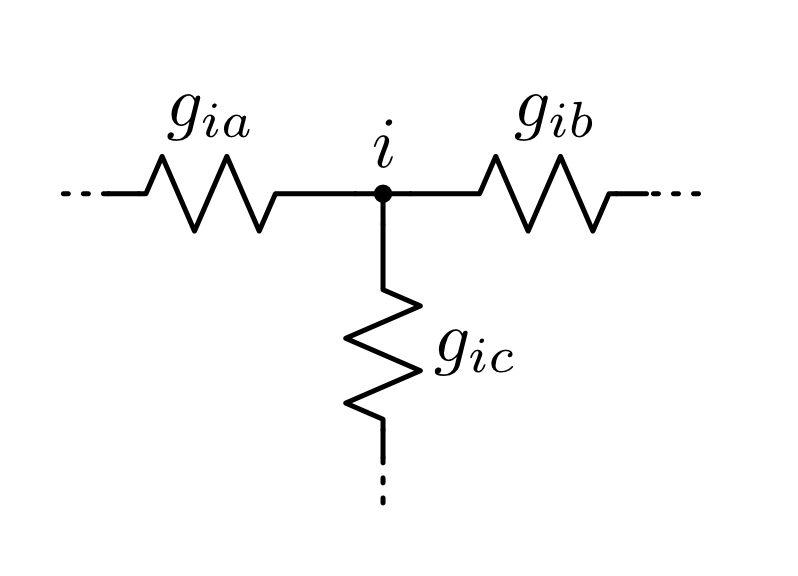
\includegraphics[width=\linewidth]{figures/circuit2.png}
  \caption{\centering Connections to group $i$ in a large percolating network.}
  \label{fig:a}
\end{subfigure}%
\begin{subfigure}{.4\textwidth}
  \centering
  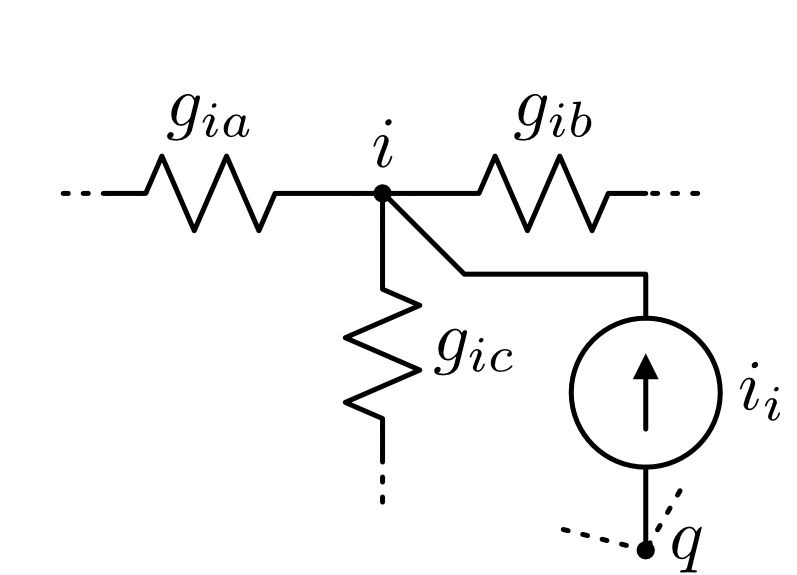
\includegraphics[width=\linewidth]{figures/circuit.png}
  \caption{\centering Connections to group $i$, with an injected current from virtual group $q$.}
  \label{fig:b}
\end{subfigure}
\caption{Setting up the system equations.}
\label{fig:viewline}
\end{figure}

\subsection{Input groups and the $G$ matrix}
An input group is a group for which we set the voltage to a known value. However, we want all unknowns on the left-hand-side and all knowns on the right-hand-side. If we multiply our known voltages by the corresponding conductances we get an injected current which can be moved to the right-hand side. Hence, we get a new system of equations

\begin{equation}\label{eq:3}
    A\vec x = G \vec v,
\end{equation}

where $\vec b = G \vec v$. Here, $\vec x$ is a vector of unknown voltages of length $m$, $A$ is an $m\times m$ condutance matrix, $\vec b$ is a vector of injected currents of length $m$, $v$ is a vector of known input voltages of length $k$, and $G$ is an $m\times k$ conductance matrix. Where $k$ is the number of inputs, then $m=n-k$.

To obtain matrix $A$ from $B$, we must remove all rows from $B$ which are input groups since the voltage $y_i$ is not in our unknown voltage vector $\vec x$. We must also remove all columns from $B$ which are input groups and add their negation to $G$. For example, if we consider Equation \ref{eq:2} where $y_a$ is an input voltage, then we rearrange to obtain
\begin{equation}\label{eq:4}
    y_i (g_{ia} + g_{ib} + g_{ic}) - y_b g_{ib} - y_c g_{ic} = y_a g_{ia}
\end{equation}
where $g_{ia}$ has been removed from $B$ on the left-hand side and will become a component of $G$ on the right-hand side. It is advantageous to maintain this $G v$ term as a means of computing $\vec b$ from our input voltages. The input voltages can, therefore, vary at each time step.

\subsection{Cholesky decomposition up/downdate}
In the case of the Cholesky decomposition, it was noted that instead of re-decomposing $A$ after a small change to the percolating network, it is possible to update the previous decomposition $LL^T$ in fewer operations. A rank-$l$ update computes the next decomposition given an update matrix $C$ with $l$ columns and $m$ rows such that the new matrix $A'=A+CC^T$. For example, in the rank-1 case, by setting two entries $i, j$ in $C$ we can change four entries in $A$ where

\begin{equation}\label{eq:5}
    CC^T = 
    \begin{bmatrix}
        \vdots\\
        a\\
        \vdots\\
        b\\
        \vdots
    \end{bmatrix}
    \begin{bmatrix}
        \cdots & a & \cdots & b & \cdots
    \end{bmatrix}
    =
    \begin{bmatrix}
        &\ddots& \vdots && \vdots\\
        & \cdots & a^2 & \cdots & ab & \cdots\\
        && \vdots &\ddots & \vdots\\
        &\cdots& ab & \cdots & b^2 & \cdots\\
        && \vdots && \vdots & \ddots
        
    \end{bmatrix}.
\end{equation}

All other entries are zeros. If we wish to increase a conductance value between $i$ to $j$ by $g$, we must add to the diagonal entries and subtract from the off diagonals at the relevant rows and columns. Hence, from Equation \ref{eq:5}, we see that $a = +\sqrt{g}$ and $b = -\sqrt{g}$. In the case we wish to decrease the conductance, we must preform a downdate where $A'=A-CC^T$ instead of an update $A'=A+CC^T$.

Multiple updates can be applied by appending column vectors together. For example, to update the connection between groups 1 and 2 by $c$ and groups 0 and 2 by $d$ we would set

\begin{equation}\label{eq:5}
    C = 
    \begin{bmatrix}
        0 & \sqrt{d}\\
        \sqrt{c} & 0\\
        -\sqrt{c} & -\sqrt{d}\\
        0 & 0
    \end{bmatrix}.
\end{equation}

For this implementation, CHOLMOD will only compute upto a rank-8 update at a time. Providing more than eight new conductance values will form multiple successive updates.

\subsection{Existing implementation}
The existing simulator using a matrix solving package called LAPACK. It finds a solution by computing the LU decomposition assuming a general matrix and preforming back substitution. At every iteration, a dense conductance-like matrix is formed which includes the input and output groups as duplicate row and column entries \cite{alex}. However, the vast majority of stored matrix entries are zero.

There are several improvements which can be made to this approach, besides the already discussed Cholesky and decomposition update methods. For large matrices, the memory requirements easily exceed the capacity of ordinary desktop machines. For example, a matrix with \num{100000} groups would require more than 75 Gb of storage. Using a sparse matrix representation will drastically reduce memory complexity to the order of megabytes. In turn, reducing the number of matrix multiplications and the amount of allocated memory will improve run times. Secondly, there is no need to reallocate memory for the matrix every iteration. Since the matrix pattern will remain consistent between runs (ie the network layout does not change), the system matrix only needs to be allocated once when the initial system is constructed. The same argument stands for the solution vector and current vector.

The existing simulator utilises BLAS, short for Basic Linear Algebra Subprograms. It is a platform independent API which takes advantage of specialised machine instructions for preforming linear algebra operations and matrix operations. Some operating systems, such as Mac OSX, ship with an optimised BLAS implementation\cite{apple}. Otherwise, projects such as OpenBLAS\cite{blas} or ATLAS\cite{atlas} allow BLAS to be installed on most systems. ATLAS optimises BLAS by running benchmarks at installation. Note that ATLAS requires disabling CPU throttling which can be difficult or impossible on systems where throttling is controlled in hardware. LAPACK, or Linear Algebra Package, is a set of solvers built on BLAS.

\section{Implementation}
A C++/C module is implemented used the CHOLMOD library as part of the SuiteSparse collection by Tim Davis et al \cite{ss}. CHOLMOD uses some parts of LAPACK as well as BLAS. CHOLMOD stands for Cholesky factorisation and modification package. The CHOLMOD library was chosen since it is specifically designed to factor sparse symmetric matrices, preform updates on those factors, and has good documentation and examples\cite{CHOLMOD}. Indeed, the default \mintinline{matlab}{A\b} operation in MATLAB will select between CHOLMOD for this case. However, MATLAB does not have a built-in update/downdate function for sparse matrices. Although a richer CHOLMOD API for MATLAB can be installed, which includes a sparse decomposition update, it was found that the matrix must be copied for each function call. The copying time was at least an order of magnitude greater than any efficiency gains from using the update/downdate method. Hence, the decision was made to pursue a C implementation. Although C++ is used to take advantage of the Standard Library, the module can be linked to C programs and the interface can be called from C programs.

Since each entry in the matrix $A$ requires a multiply operation when solving the system, the amount of memory used by $A$ is proportional to the time it takes to solve. Hence, a sparse representation of $A$ and $G$ are constructed in this implementation. Another advantage is that large sparse matrices have lower RAM requirements than their dense counterparts. However, constructing test matrices in compressed column form becomes more difficult to achieve without constructing a full dense matrix as an intermediate step; doing so would require $n^2$ memory at startup, a limiting factor for large matrices. Here, a method is developed for constructing a sparse representation from a triplet using memory proportional to the number of non-zero entries in the matrix. For matrices of tight bandwidth, the number of non-zeros is approximately proportional to $n$.

 The easiest way to describe the algorithms and data structures used is with a simple example. However, remember that in practice these networks can be around $10^5$ groups in size and their matrix representations are predominantly zero-entries. Consider the simple network in Figure \ref{fig:3}. The conductance matrix of this network can be found as shown in Equation \ref{eq:6}.

\begin{figure}[!htbp]
    \centering
    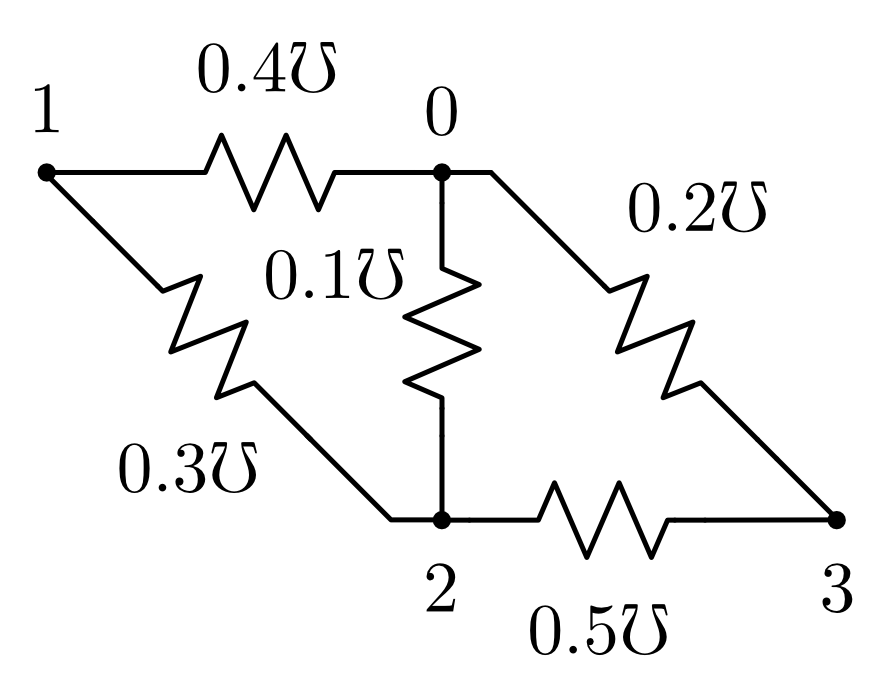
\includegraphics[width=0.33\linewidth]{figures/circuitsimp.png}
    \caption{Example system.}
    \label{fig:3}
\end{figure}

\begin{equation}\label{eq:6}
    B =
    \begin{bmatrix}
    0.7 & -0.4 & -0.1 & -0.2\\
    -0.4 & 0.7 & -0.3 & 0\\
    -0.1 & -0.3 & 0.9 & -0.5\\
    -0.2 & 0 & -0.5 & 0.7
    \end{bmatrix}
\end{equation}

\subsection{Inputting data using .mtx and triplets}
The network configuration is assumed to be provided to the module in the form of a triplet. A CHOLMOD triplet object consists of three arrays: the start group index, the end group index, and the conductance value. In other words, the $i$th entry of these arrays tells us the conductance between two groups. A triplet object can be populated from a \mintinline{text}{.mtx} text file. However, this \mintinline{text}{.mtx} must be square and in coordinate symmetric lower triangular form with real value entries. Symmetric lower triangular means that we only store a connection from $i$ to $j$ and not $j$ to $i$, due to the symmetry of $B$. In lower triangular form, a coordinate $(i, j)$ is stored only if $i > j$, ie the row index is strictly greater than the column index. The triplet for our simple example would appear as follows,

\begin{equation}
    \begin{bmatrix}
    \text{start group}\\
    \text{end group}\\
    \text{conductance}
    \end{bmatrix}=
    \begin{bmatrix}
    3 & 3 & 2 & 2 & 1\\
    2 & 0 & 1 & 0 & 0\\
    0.5 & 0.2 & 0.3 & 0.1 & 0.4
    \end{bmatrix}.
\end{equation}

Code which exports \mintinline{text}{.mtx} files can be found online. However, \mintinline{text}{.mtx} files are often produced in the wrong format. A helper function is provide with the module to convert coordinate \mintinline{text}{.mtx} files into the form specified above. A \mintinline{text}{.mtx} file is probably in the correct format if it begins with the line

\begin{minted}{text}
%%MatrixMarket coordinate real symmetric
\end{minted}

\subsection{Adjacency lists}
The incoming triplet is sorted by column and secondarily by row using insertion sort. Insertion sort was chosen since it is easy to write and also because the triplet is likely to be in almost sorted order. If you are building .mtx files, it is recommended you write the entries in the same order. A sorted triplet ensures that the adjacency lists remain ordered for when the sparse matrices are constructed, which require sorted columns. Column-wise and row-wise adjacency lists are constructed from the triplet. Note that only the column-wise adjacency lists contain the diagonal entries. The additional row-wise adjacency lists are a consequence of storing only the lower triangular entries in the triplet. This means if we want to extract an entire column (including above the diagonal), we have to search through all the lists of pairs to find the entries along a row. It is required that we extract columns when constructing the $G$ matrix. The column-wise adjacency list is easily converted into a symmetric compressed column form, the sparse representation of $A$.

Example adjacency lists are shown in Figure \ref{fig:adj}. The column-wise adjacency list is structured such that the $j$th index (column) contains a list of pairs. Each pair contains the row index $i$ and the corresponding conductance value at that index. The row-wise adjacency lists are similar, except the $i$th index (row) has a list of pairs containing the column $j$ and the conductance.

\begin{figure}[!htbp]
\centering
\begin{subfigure}{.5\textwidth}
  \centering
  \begin{minted}[linenos=0]{text}
0: (0, 0.7) (1, -0.4) (2, -0.1) (3, -0.2) 
1: (1, 0.7) (2, -0.3) 
2: (2, 0.9) (3, -0.5) 
3: (3, 0.7) 
  \end{minted}
  \caption{\centering Column-wise adjacency lists.}
  \label{fig:c}
\end{subfigure}%
\begin{subfigure}{.5\textwidth}
  \centering
    \begin{minted}[linenos=0]{text}
0: 
1: (0, -0.4) 
2: (0, -0.1) (1, -0.3) 
3: (0, -0.2) (2, -0.5) 
  \end{minted}
  \caption{\centering Row-wise adjacency lists.}
  \label{fig:d}
\end{subfigure}
\caption{Example adjacency lists.}
\label{fig:adj}
\end{figure}

\subsection{Sparse representation}
CHOLMOD stores its matrices in Compressed Column form (CCF), as does MATLAB. This form is convenient for being both space efficient and computationally efficient for matrix operations. The sparse representation of our example is,

\begin{equation}\label{eq:n}
    \begin{bmatrix}
    \text{column pointers}\\
    \text{row indices}\\
    \text{conductances}
    \end{bmatrix}=
    \begin{bmatrix}
    0 & 4 & 6 & 8 & 9\\
    0 & 1 & 2 & 3 & 1 & 2 & 2 & 3 & 3\\
    0.7 & -0.4 & -0.1 & -0.2 & 0.7 & -0.3 & 0.9 & -0.5 & 0.7
    \end{bmatrix}.
\end{equation}

It is helpful to compare the entries below and along the diagonal in Equation \ref{eq:6} when understanding CCF. In the list of column pointers, each entry $i$ is an index in the other two lists to the beginning of column $i$. The integers in the row indices list which follow from this index are the rows at which there is an entry in the current column. The corresponding conductance value is then stored in the conductances list. From the adjacency lists, the matrices $A$ and $G$ are easily constructed in sparse form. A helpful consequence of storing the matrices in this form is that the diagonals are always the first item in each column. Hence, it is easy to find and update these values during initial matrix formation and while updating conductance entries. Otherwise, finding a specific entry in a column may involve a binary search.

The additional term in the column pointers vector is not a column pointer. The value 9 is the number of non-zero entries \emph{stored} in compressed column form, In other words, it is the length of the row indices and conductances vectors. Adding the length is a convention which make it simpler for an algorithm to calculate the number of entries in a column if iterating though columns.

\section{Further work}

\begin{enumerate}
    \item Verification. Although the solver has been tested on the above case, it requires more rigorous testing some larger matrices.
    \item Benchmarking. Feed the same matrices into the existing solver and this solver to compare their performance. Hopefully this one is noticably faster, especially for larger matrices. Also see the Tuning section.
    \item Integration. Provided the solver works well, consider integrating it into the existing simulator or rebuilding a new simulator around this solver.
\end{enumerate}

\subsection{Other noteworthy points}

\begin{itemize}
    \item If a new simulator is on the cards, I would recommend using C++ to take advantage of the STL and storing connections in an adjacency list similar to the one used in solve.cpp. If so, it would also be possible to build this adjacency list and pass it in directly to solve.cpp (with some API modifications). Doing so would save on the initial build time if it becomes an issue. A big advantage is that C++ STL structures manage their own memory, so realloc is not needed.
    \item There are three lookup tables used heavily in the main loop as part of the update operation. It is possible that an speed gain could be obtained by instead using a much smaller list and doing a binary search on this list. I suspect this since, as the lookup tables become larger, they will be constantly moving in and out of cache. Assuming a small number of input groups, it would be possible to replace these lookup tables with a simple computation which may end up being faster if less memory is moving around. The best way to know if this method provides an improvement is probably to test it.
    \item It would be worth researching the Newton-Raphson method, how it works, and if it would be applicable here. Especially if we wish to include capacitance into the model.
    \item If the solver is giving incorrect values sometimes, then it is possible that I have missed a permutation conversion. The CHOLMOD library computes its own permutation vector, but sometimes arguments are supplied to functions permuted and sometimes they are not. I would recommend reading through the CHOLMOD documentation and checking the argument matrices to each CHOLMOD call in this case.
\end{itemize}

\subsection{Tuning}
There are two variables which are currently set to arbitrary values.

\mintinline{text}{UPDATE_LIMIT} in \mintinline{text}{solver_iterate_ac} specifies the number of conductance updates at which it is no longer worth using the Cholesky update method. For example, if close-to-all of the conductances are updated then it is probably faster to obtain the $LDL^T$ factorisation directly from $A$ instead of updating the previous factorisation. Hence, if the number of conductance updates is greater-or-equal-to \mintinline{text}{UPDATE_LIMIT} then the factorisation is obtained from $A$. Otherwise, the new factorisation is obtained by updating the previous factorisation, which should be faster for small numbers of updates.

\mintinline{text}{DECOMPOSITION_FREQUENCY} in \mintinline{text}{solve.h} is the number of iterations after which we should recalculate the factorisation from $A$. This option is added in case precision errors become an issue after a large number of Cholesky updates. However, it may turn out that this is not a problem at all.

In the case that we do not need to set a \mintinline{text}{DECOMPOSITION_FREQUENCY} and it is not worthwhile setting an \mintinline{text}{UPDATE_LIMIT}, then we no longer have the need to update the $A$ matrix and $G$ matrix at each iteration. Hence, the code responsible for these updates could be removed to improve performance.

\newpage
% \nocite{*}
\bibliographystyle{IEEEtran}
\bibliography{references}

\end{document}
